\chapter{Entwicklung}\label{Entwicklung}

\section{Anforderungen}\label{sec:Anforderungen}

\section{Konzeptentwurf}\label{sec:Konzeptentwurf}

\section{Implementierung}\label{sec:Implementierung}

\section{Tests}\label{Tests}
Während der Entwicklung wurde mit Hilfe von ausführlichen Tests die Funktionalität neuer Features sichergestellt und eine ausführliche Testdokumentation angefertigt. Dadurch sollten Fehler, Probleme und mögliche Verbesserungen entdeckt und festgehalten werden. \\
Das Ziel war es für jedes neue Feature einen Test durchzuführen.\\


\subsection{Testdurchführung}
Bei der Testdurchführung wurde darauf Wert gelegt, dass die einzelnen Durchläufe in der selben Testumgebung und unter den gleichen Umständen stattfinden, um eine Vergleichbarkeit zwischen den verschiedenen Versionen herzustellen.
So konnte nach jedem Test zusätzlich festgestellt werden, ob sich eventuell die bestehende Eigenschaften im Vergleich zur Vorgängerversion verschlechtert oder verbessert hatten. \\
Zu diesem Zweck wurde für jeden Durchlauf der in Abbildung \ref{fig:Testaufbau} gezeigte Versuchsaufbau gewählt.

\begin{figure}[h!]
\centering
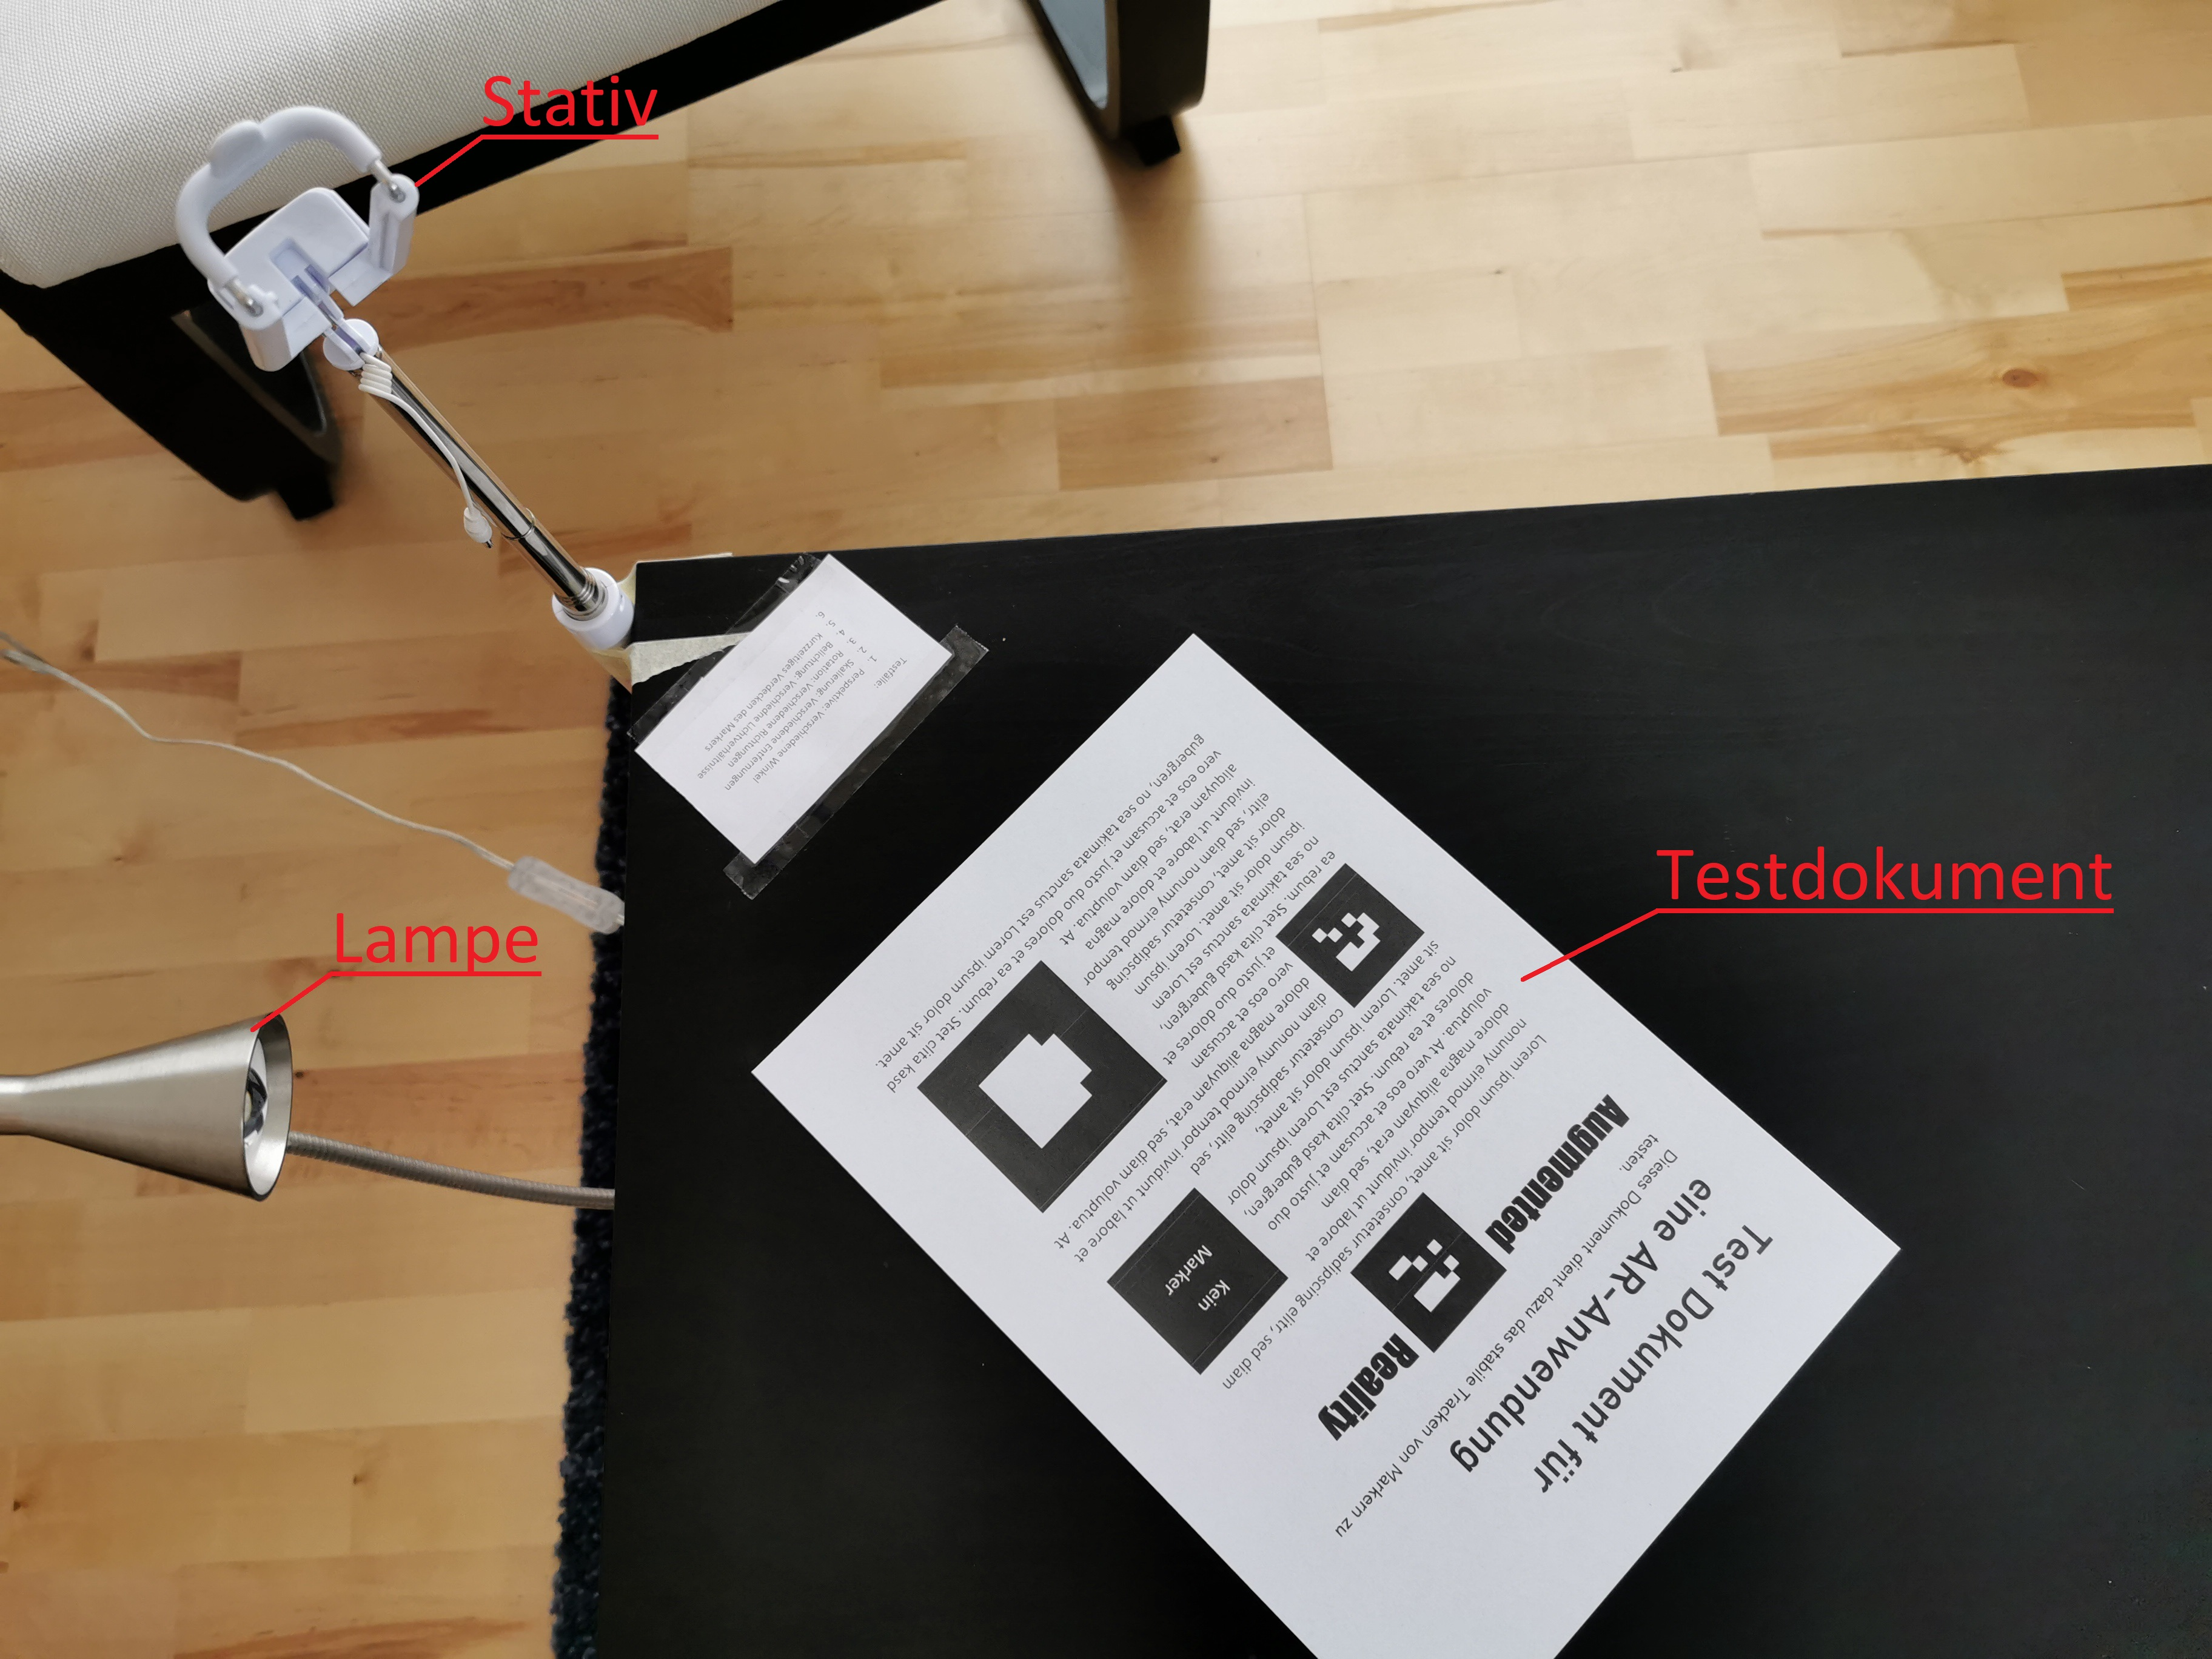
\includegraphics[width=0.7\textwidth]{Abbildungen/Testaufbau.jpeg}
\caption[Testaufbau]{Der Testaufbau für jeden Durchlauf. (Quelle: Eigene Darstellung)}
\label{fig:Testaufbau}
\end{figure}

Da der Prototyp in Android Studio entwickelt wurde, war es zudem möglich die Anwendung direkt auf einem Androidendgerät zu testen. Dieses bot die Möglichkeit die Tests in einer realistischen, praxisnahen Umgebung durchzuführen und demzufolge noch bessere Erkenntnisse über die Alltagstauglichkeit der neuen Features zu erhalten.  \\
Dafür wurde bei jedem Durchlauf ein Huawei P30 Pro genutzt und das Tracking wurde anhand eines dafür angefertigten Dokumentes \todo{Verweis auf Testdokument(Anhang)} getestet. Dieses Dokument wurde im Laufe der Entwicklung an die neuen Features angepasst und optimiert. Grundlegend bildet das Dokument einen oder mehrere Marker ab. Gegebenenfalls sind die Marker in Textpassagen eingebunden, um den Schwierigkeitsgrad für die Markererkennung zu erhöhen.\\
Während des Testlaufs wurden jedes mal vier Testfälle durchlaufen, die in Abschnitt \ref{sec:Testfälle} beschrieben werden. Dabei wurden sowohl die Neuerungen getestet, als auch Veränderungen in den bereits bestehenden Features festgehalten.\\
Jeder Testfall wurde dabei mit Hilfe der in Android enthaltenen Funktion \glqq Bildschirmrekorder\grqq aufgezeichnet und in dem entsprechenden Testbericht dokumentiert.


\subsection{Testfälle}\label{sec:Testfälle}
Die Testfälle wurden von den relevanten Eigenschaften des Feature Trackings abgeleitet und konnten auch auf das Marker Tracking angewendet werden. \todo{Zitieren von der Medieninformatikvorlesung}
Insgesamt wurden die folgenden vier Testfälle herausgearbeitet:
\begin{itemize}
\item Perspektivische Invarianz: Dieser Testfall diente dazu das Tracking aus verschiedenen Perspektiven zu testen. Dazu wurde die Kamera auf das Testdokument gerichtet und anschließend der Winkel zum Dokument so verändert das verschiedenen, perspektivische Verzerrungen der Marker erzeugt wurden.

\begin{figure}[H]
	\centering
    
\includegraphics[width=0.2\textwidth]{Abbildungen/Invarianz/Perspektive1.jpg}
    
\includegraphics[width=0.2\textwidth]{Abbildungen/Invarianz/Perspektive2.jpg}
    \caption{Perspektivische Verzerrung eines Markers. (Quelle: Eigene Darstellung)}
\end{figure}

\item Skalierungsinvarianz: Dieser Testfall diente dazu das Tracking aus verschiedenen Entfernungen zu testen. Dazu wurde die Kamera langsam auf das Testdokument zu- und wegbewegt, um verschiedenen Markergrößen bzw. -auflösungen zu erhalten.

\begin{figure}[H]
    \centering
    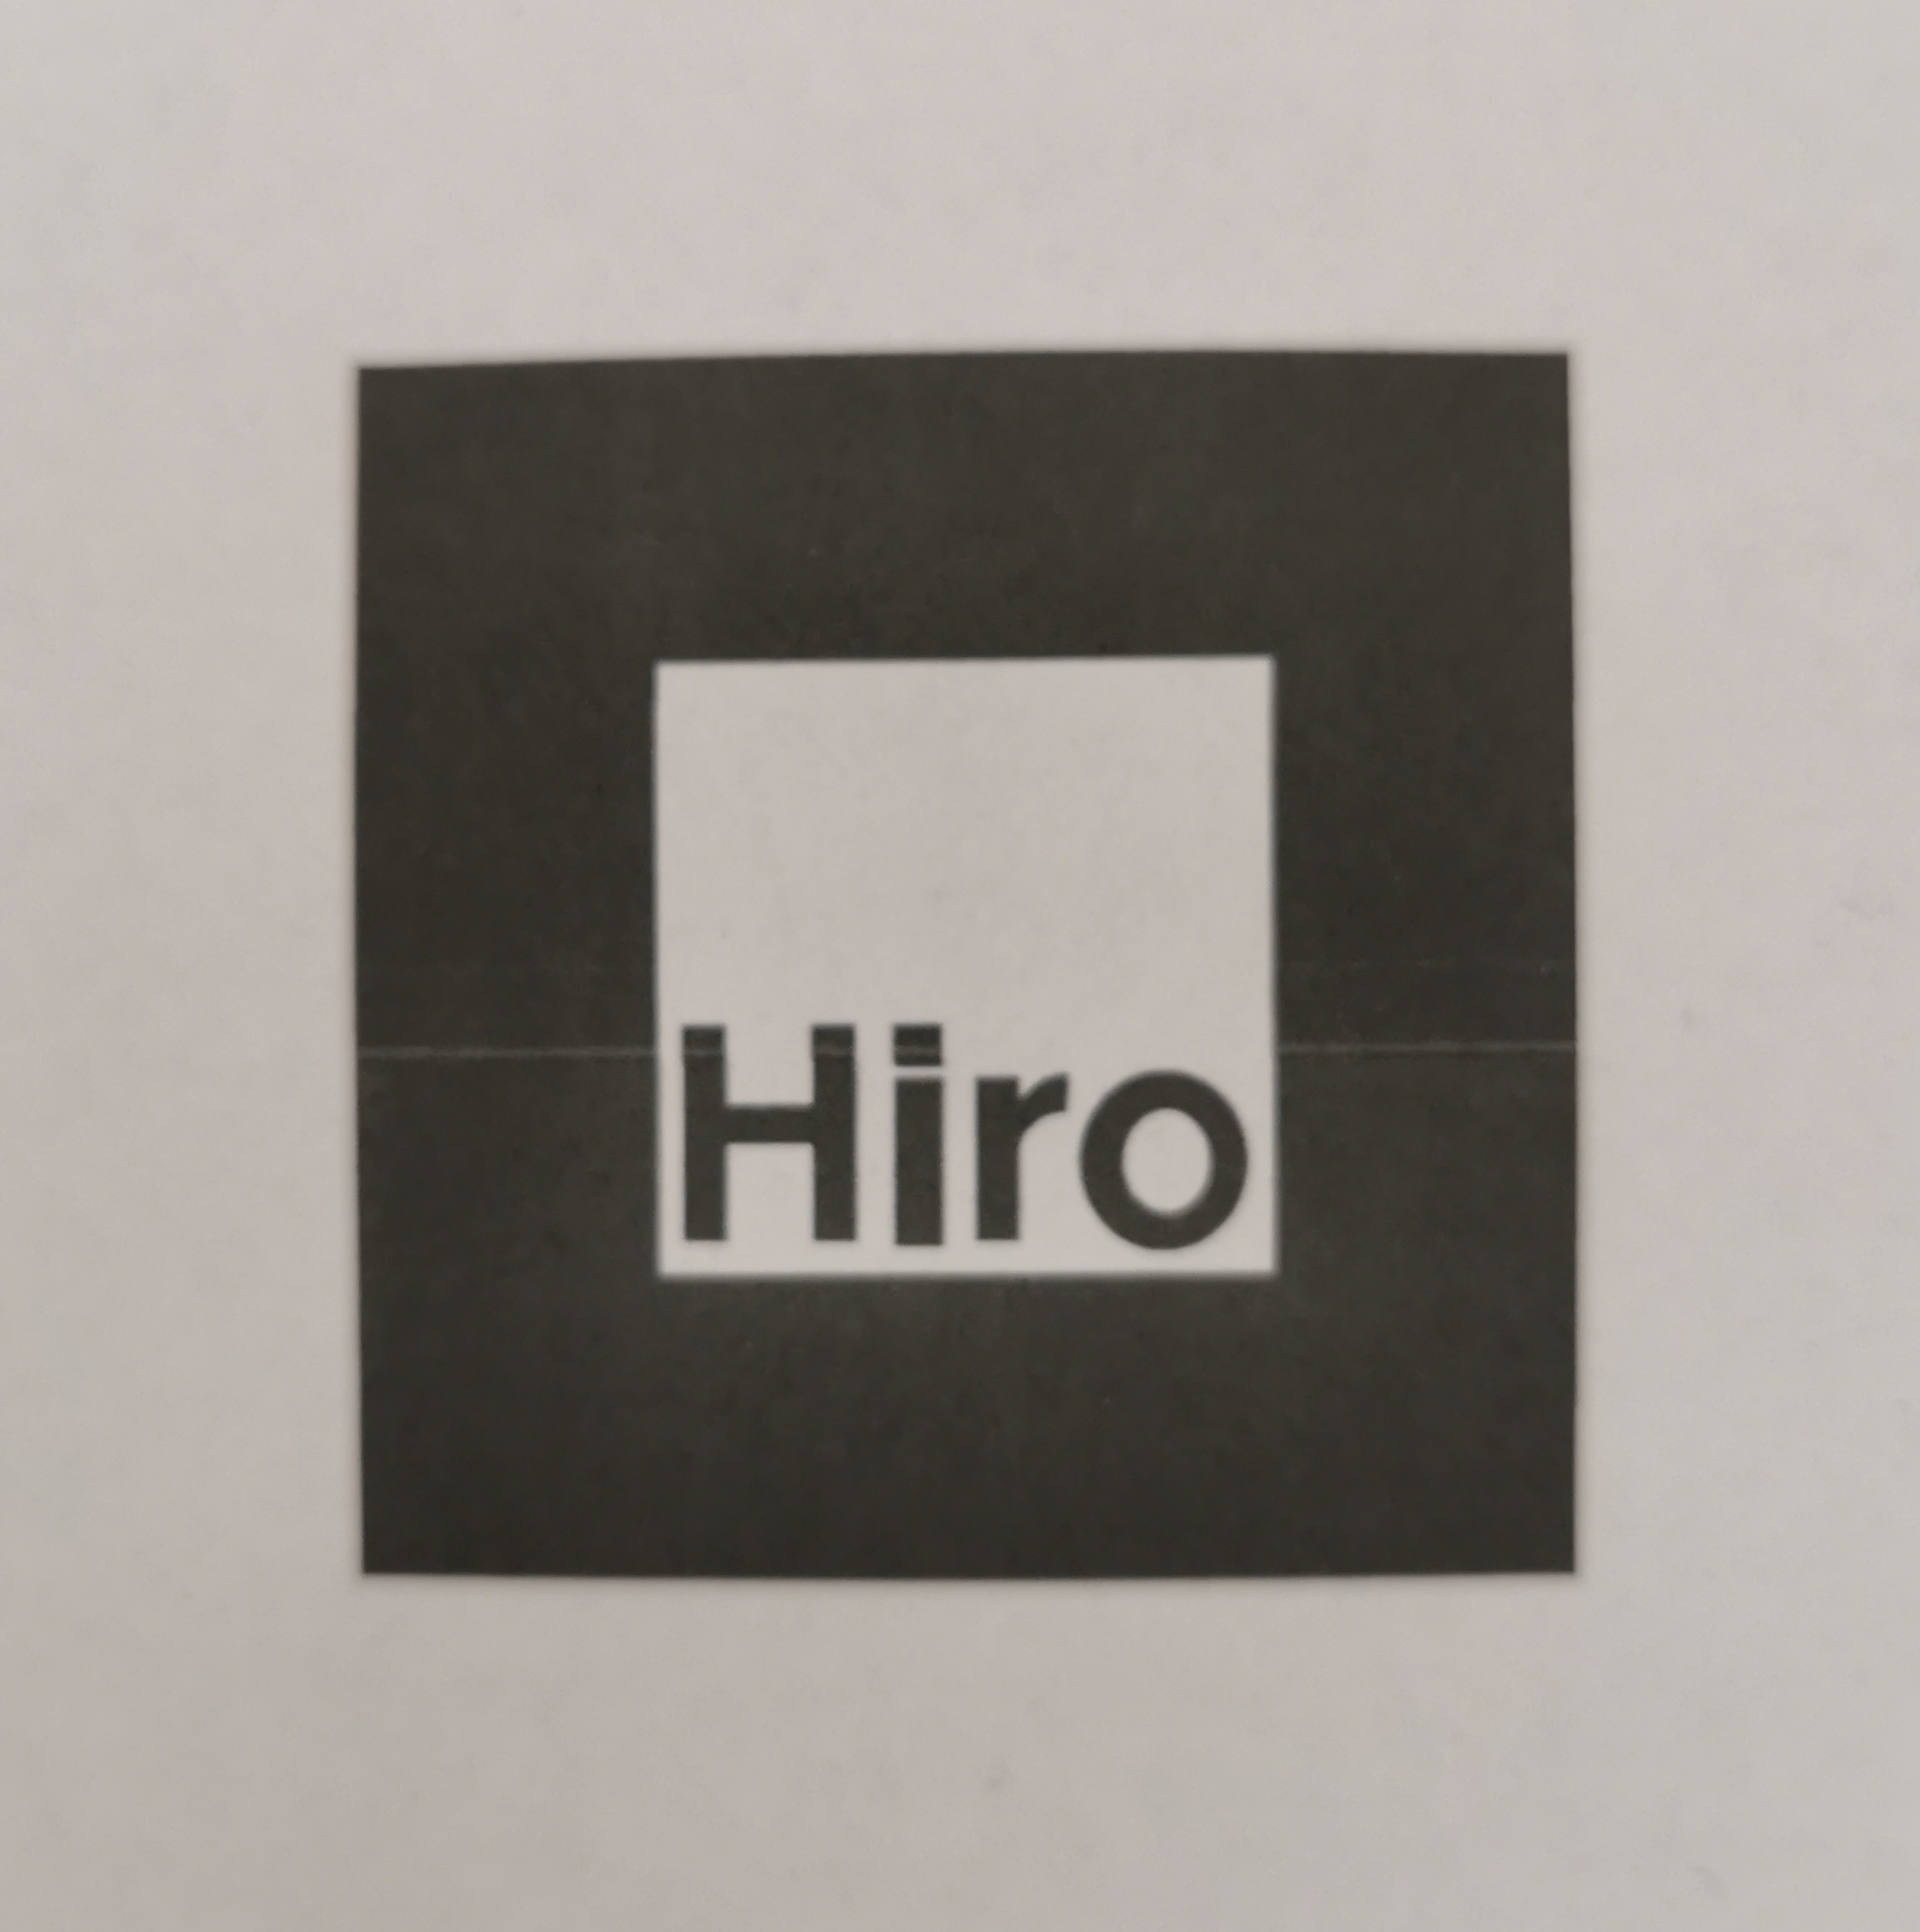
\includegraphics[width=0.2\textwidth]{Abbildungen/Invarianz/Skalierung1.jpg}
    
\includegraphics[width=0.2\textwidth]{Abbildungen/Invarianz/Skalierung2.jpg}
    \caption{Verschiedene Skalierungen eines Markers. (Quelle: Eigene Darstellung)}
\end{figure}

\item Rotationsinvarianz: Dieser Testfall diente dazu das Tracking von Markern mit unterschiedlichen Rotationen zu testen, dazu wurde die Kamera auf das Dokument gerichtet und anschließend wurde letzteres langsam rotiert, um zu evaluieren, ob die Marker auch mit unterschiedlichen Rotationen korrekt erkannt werden.
\begin{figure}[H]
    \centering
    
\includegraphics[width=0.2\textwidth]{Abbildungen/Invarianz/Rotation1.jpg}
    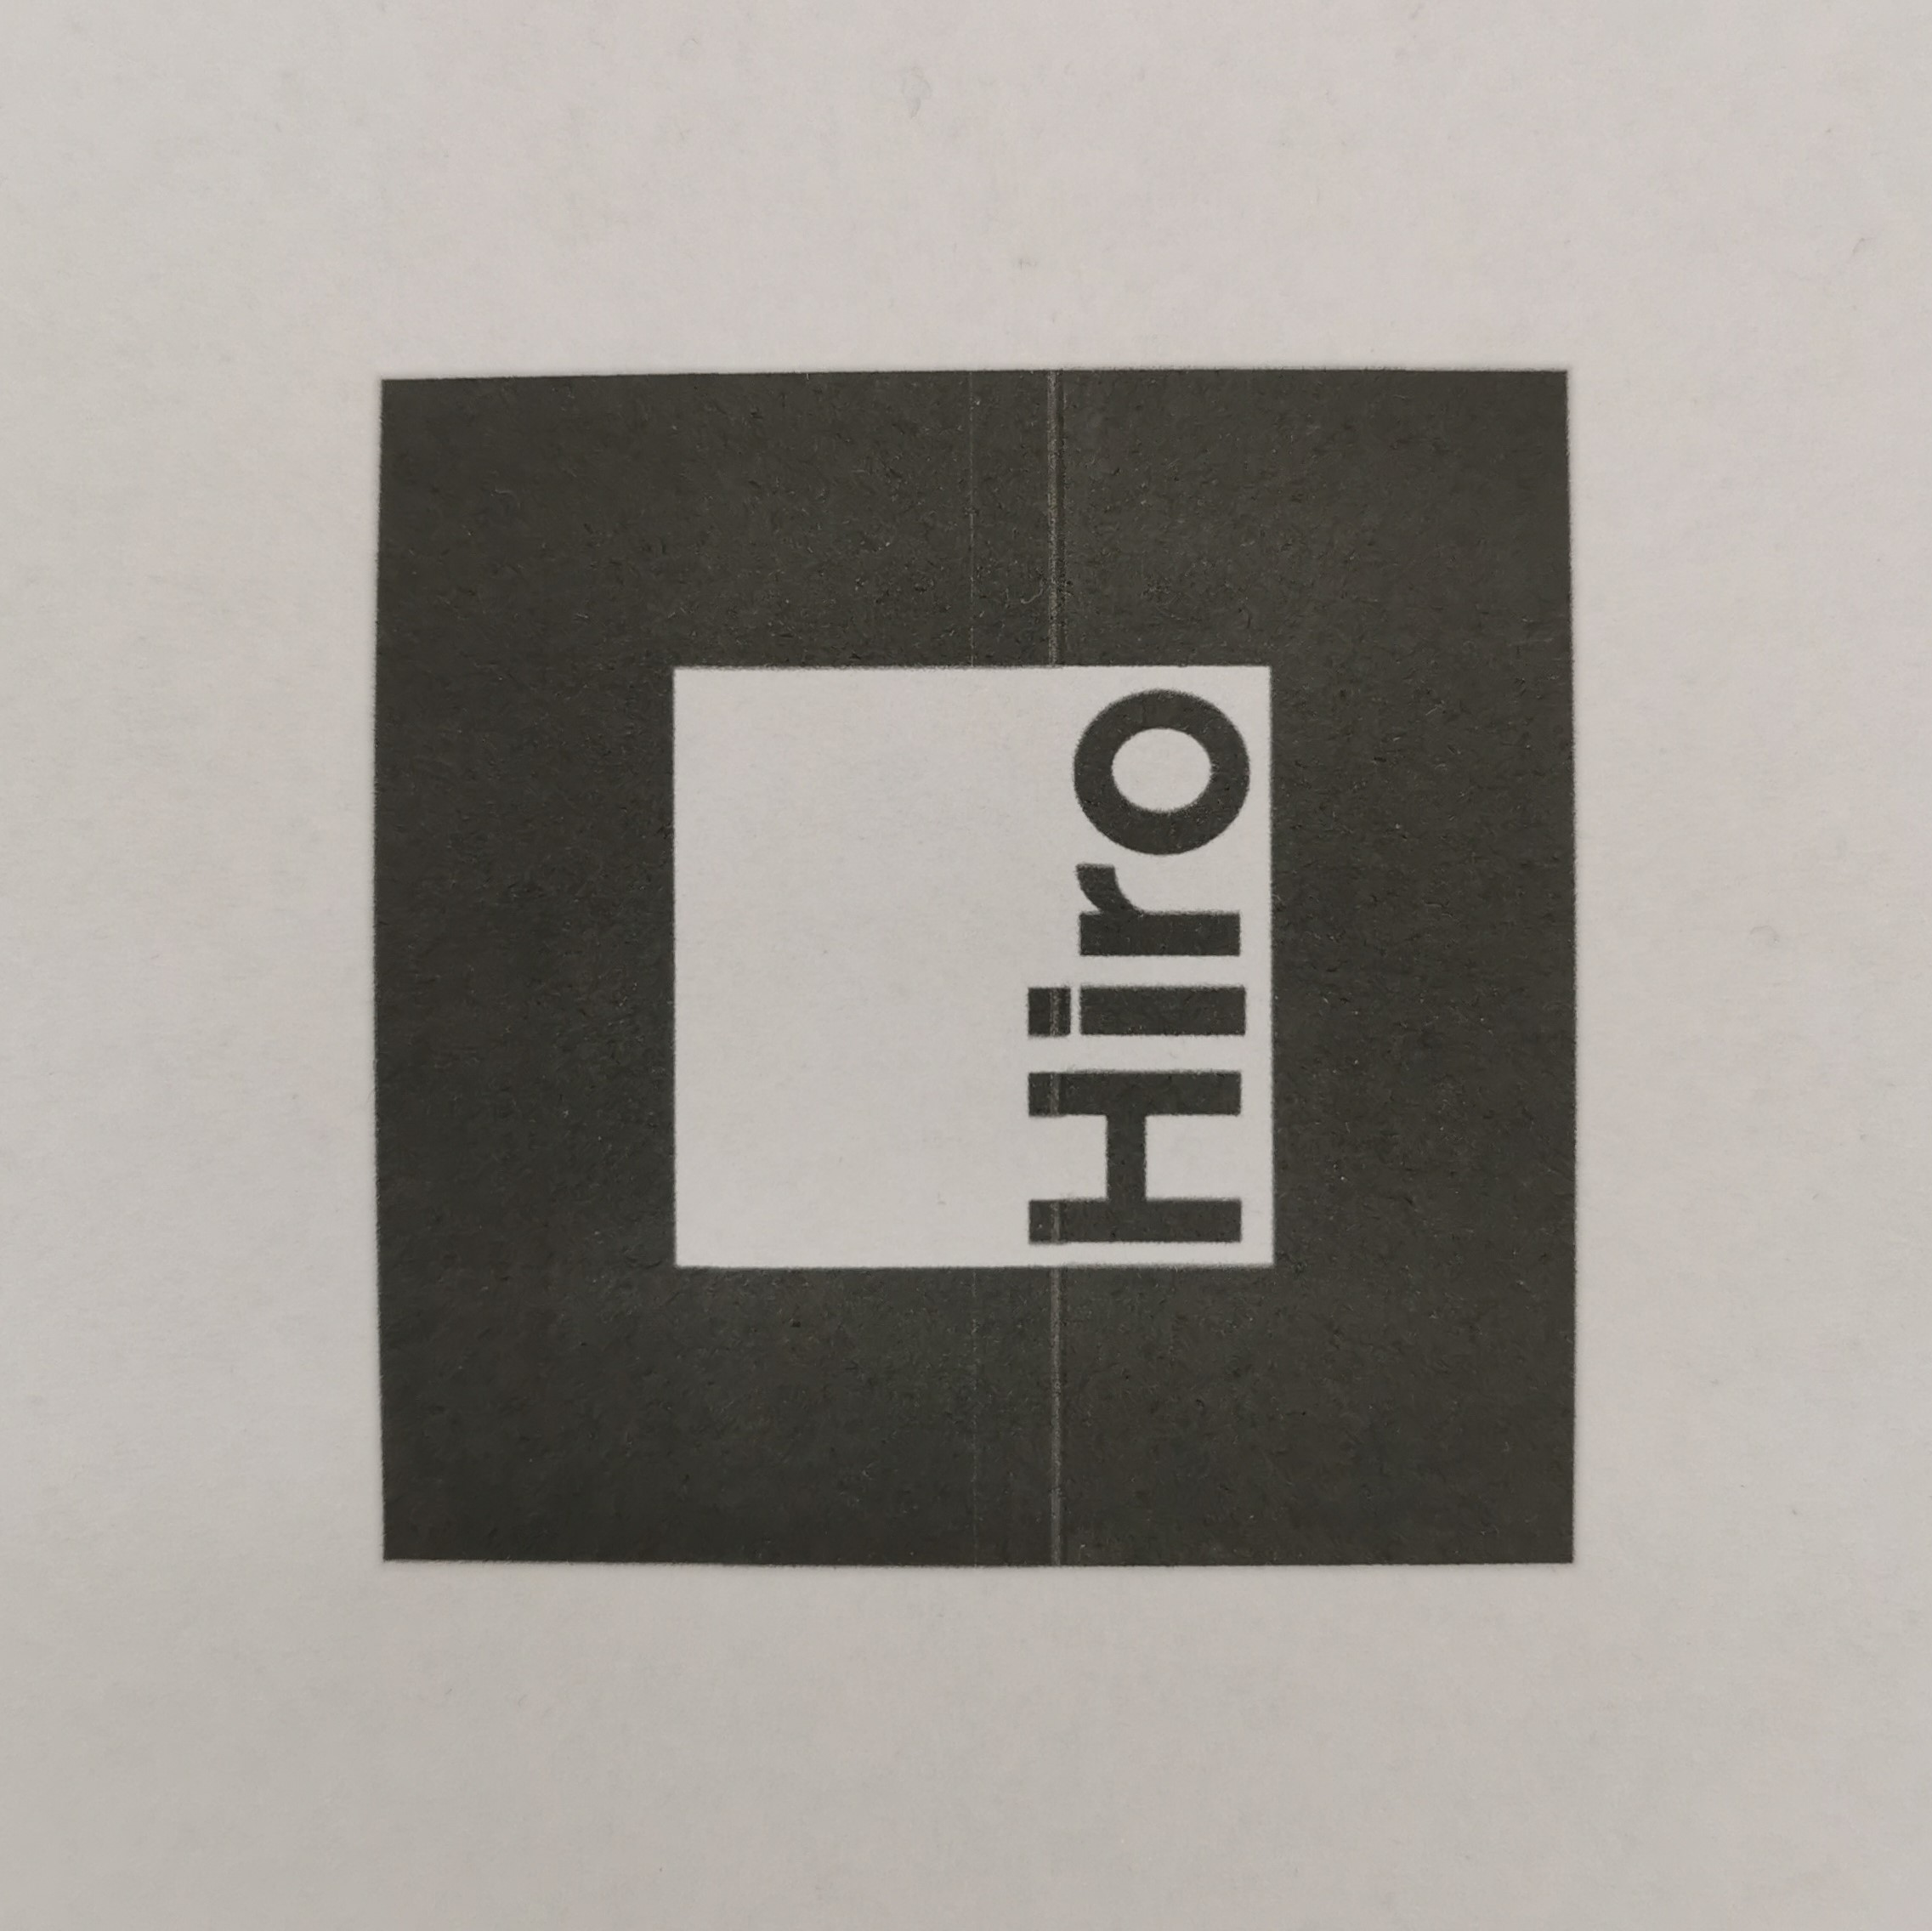
\includegraphics[width=0.2\textwidth]{Abbildungen/Invarianz/Rotation2.jpg}
    \caption{Verschiedene Rotationen eines Markers. (Quelle: Eigene Darstellung)}
\end{figure}

\item Belichtungsinvarianz: Dieser Testfall diente dazu das Tracking von Markern gegenüber unterschiedlichen Belichtungen zu testen. Dazu wurde mit Hilfe einer Lampe die Belichtung des Testdokumentes verändert.
\begin{figure}[H]
  	\centering
    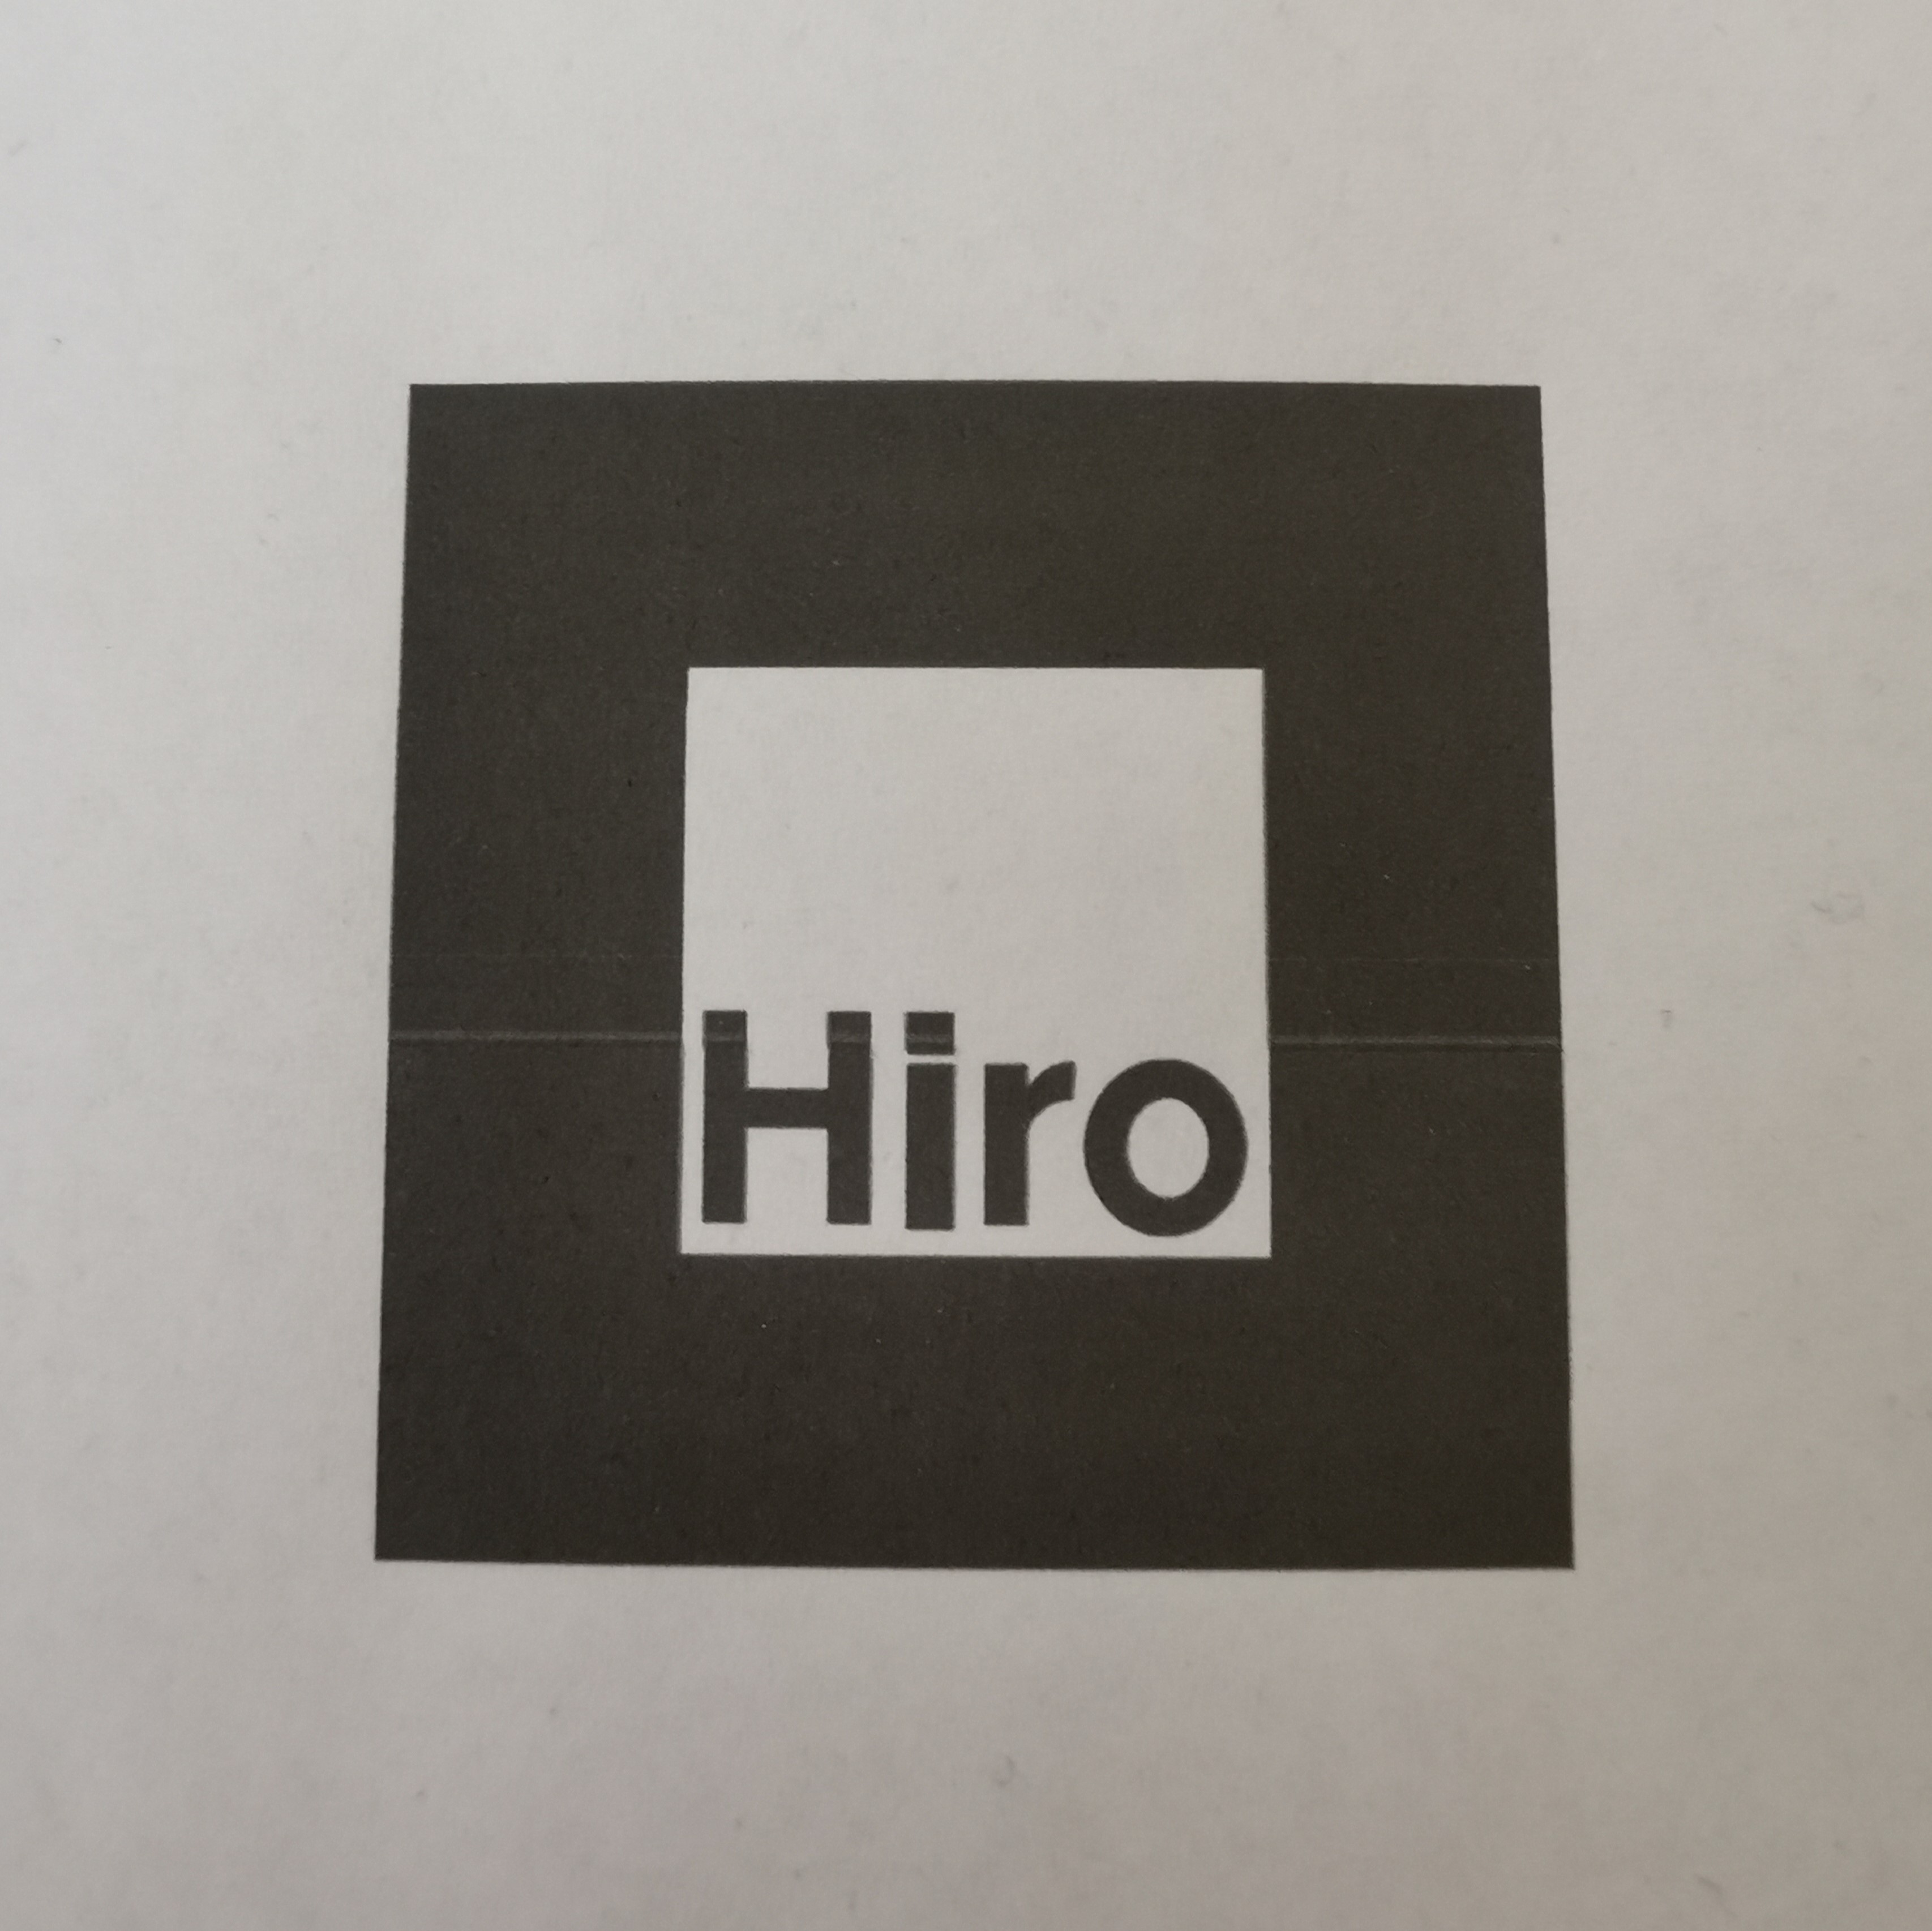
\includegraphics[width=0.2\textwidth]{Abbildungen/Invarianz/Belichtung1.jpg}
    
\includegraphics[width=0.2\textwidth]{Abbildungen/Invarianz/Belichtung2.jpg}
    \caption{Verschiedene Belichtungen eines Markers. (Quelle: Eigene Darstellung)}
\end{figure}

\item  Trackinggeschwindigkeit:\todo{Besserer Name} Dieser Testfall sollte die Geschwindigkeit des Trackings, sowie die Robustheit testen. Dazu wurden ein oder mehrere Marker kurzzeitig mit der Hand verdeckt, um zu testen,ob anschließend alle Marker wieder erfolgreich getrackt wurden und wie schnell dieses erfolgte.

\end{itemize}
Eine weitere, aus dem Feature Tracking bekannte Eigenschaft wäre die Invarianz gegenüber partieller Verdeckung gewesen, diese wurde jedoch nicht getestet, da zu Beginn in den Anforderungen ein vollständig erkannter Marker voraus gesetzt wurde.\\
All diese Testfälle beziehen sich auf das Marker Tracking, während dessen konnten jedoch auch das Rendern des Modells und weitere Features die nicht direkt mit dem Tracking zusammenhängen getestet werden.\\

\subsection{Zusammenfassung}
\todo{Am Ende schreiben}
- Belichtung nicht einfach zu testen
- starke Belichtungswechsel teilweise kurze Aussetzer

